\documentclass{article}%
\usepackage[T1]{fontenc}%
\usepackage[utf8]{inputenc}%
\usepackage{lmodern}%
\usepackage{textcomp}%
\usepackage{lastpage}%
\usepackage[head=40pt,margin=0.5in,bottom=0.6in]{geometry}%
\usepackage{graphicx}%
%
\title{\textbf{Lorent Saleh: Cronología de un preso político}}%
\author{El Nacional Web}%
\date{12/10/2018}%
%
\begin{document}%
\normalsize%
\maketitle%
\textbf{URL: }%
http://www.el{-}nacional.com/noticias/presos{-}politicos/lorent{-}saleh{-}cronologia{-}preso{-}politico\_255547\newline%
%
\textbf{Periodico: }%
EN, %
ID: %
255547, %
Seccion: %
Presos políticos\newline%
%
\textbf{Palabras Claves: }%
Política, Presos políticos, Sebin\newline%
%
\textbf{Derecho: }%
1.2, %
Otros Derechos: %
1.10, %
Sub Derechos: %
1.2.2, 1.10.1\newline%
%
\textbf{EP: }%
NO\newline%
\newline%
%
\textbf{\textit{El dirigente estudiantil fue extraditado y entregado al Sebin en el año 2014 por el gobierno de Juan Manuel Santos}}%
\newline%
\newline%
%
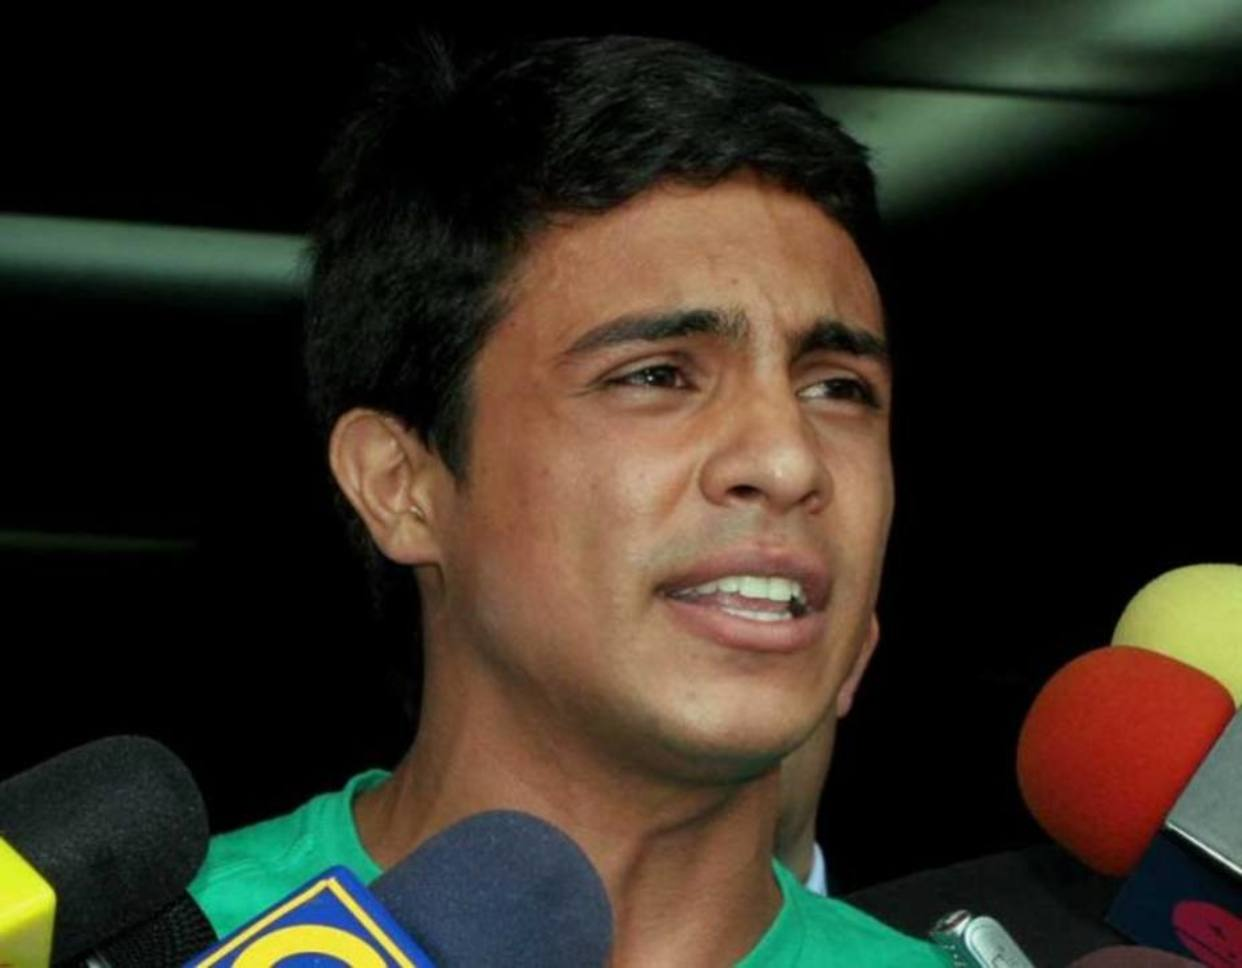
\includegraphics[width=300px]{111.jpg}%
\newline%
%
Lorent Saleh, preso político desde 2014, cumplió en septiembre cuatro años detenido luego de que fuese deportado a Venezuela por el gobierno colombiano por presuntamente realizar actividades que atentaban contra la seguridad nacional, el orden público, la salud pública, la tranquilidad social, la seguridad pública.%
\newline%
%
La extradición del dirigente estudiantil por el gobierno del presidente Juan Manuel Santos fue rechazada en su momento por el ex mandatario colombiano Álvaro Uribe Vélez, el cual indicó que la decisión buscaba complacer a las Fuerzas Armadas Revolucionarias de Colombia (Farc) y al gobierno venezolano.%
\newline%
%
“Santos entrega estudiante a Maduro mientras este protege terroristas cuya extradición Santos no pide. Siempre buscan complacer a Farc y a Maduro”, publicó Uribe en~ su Twitter luego de conocer la extradición de Saleh.%
\newline%
%
El estudiante, que es acusado por el gobierno de Nicolás Maduro de estar vinculado con paramilitares colombianos y de planear actividades golpistas y terroristas en suelo venezolano, permanece recluido en la sede del Servicio Bolivariano de Inteligencia Nacional (Sebin).%
\newline%
%
Desde su detención, en 2014, la audiencia preliminar en tribunales de Saleh ha sido pospuesta en 53 oportunidades entre otras razones por la negativa del Sebin a trasladarlo a los juzgados para que inicie la causa en su contra.%
\newline%
%
Debido a la lucha por la defensa de los Derechos Humanos y la libertad en Venezuela emprendida por Saleh, en el año 2017 el Parlamento Europeo decidió concederle el Premio Sájarov, el cual fue recibido por su madre en Bélgica.%
\newline%
%
Luego de cuatro años de detención, permancer durante 26 meses recluido en "La Tumba" y ~la muerte de Fernando Albán, concejal al municipio Libertador de Caracas, en circunstancias aún por esclarecer, que se encontraba detenido por el Sebin, el gobierno anunció este viernes la excarcelación de Lorent Saleh por presuntamente mostrar “conductas violentas, destructivas y suicidas”. Como parte de la medida de excarcelación, el gobierno ordenó que Saleh abandonara el país y se “trasladara” a España, situación que fue calificada por dirigentes opositores como una orden de destierro.%
\newline%
%
\end{document}